O tym czy firewall w systemie ubuntu jest potrzebny czy nie można długo dysktuować. Jeżeli dla spokoju ducha potrzebujesz działającej ściany ogniowej to Ubuntu oferuje proste narzędzie do zarzadzania wbudowanym w system operacyjnym programem iptables.

GUFW (\textcolor{ubuntu_orange}{GUI for Uncomplicated FireWall} znajduje się w repozytoriach Ubuntu. Zainstaluj go przez Centrum Oprogramowania (,,Konfiguracja zapory Firewall'') lub za pomocą terminala:
\begin{lstlisting}[language=bash]
sudo apt-get install gufw
\end{lstlisting}

\begin{wrapfigure}{R}{0.5\textwidth}
	\vspace{-10pt}
	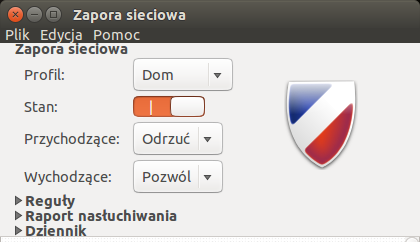
\includegraphics[width=\linewidth]{images/programy_gufw.png}
\end{wrapfigure}

Uruchom program GUFW. Konfiguracja zapory sieciowej wymaga uprawnień administratora, zostaniesz poproszony o uwierzytelnienie się. Kiedy to zrobisz, otwarte zostanie główne okno programu.

Domyślnie zapora jest wyłączona. Kliknij na przycisk przy pozycji \textcolor{ubuntu_orange}{Stan} i ustaw go na włączony (tak jak na rysunku). Od tego momentu firewall działa i będzie automatycznie się uruchamiać wraz ze startem systemu. Warto jeszcze przestawić \textcolor{ubuntu_orange}{Przychodzące} z pozycji ,,Odmów'' na ,,Odrzuć''\footnote{Kiedy ktoś będzie próbował się połączyć z zewnątrz to zamiast otrzymać sygnał ,,zajęty'' dostanie ,,głuchy telefon''}. Teraz firewall jest skonfigurowany według ogólnie przyjętego na świecie schematu dla komputerów osobistych: odrzuć wszystkie połączenia przychodzace, zezwól lokalnym programą na łączenie się z internetem.

\subsubsection{Dodawanie reguł}
Kiedy masz już ustaloną politykę działania firewalla, może się zdażyć iż potrzebujesz wprowadzić jakiś wyjątek. Zrobisz to w zakładce \textcolor{ubuntu_orange}{Reguły}. Aby dodać regułę kliknij na przycisk + znajdujący się pod tabelą. Są trzy sposoby na stworzenie reguły:
\begin{itemize}
\item \textcolor{ubuntu_orange}{Predefiniowana} --- pozwala stworzyć regułę w oparciu o szablon. Jeżeli potrzebujesz zablokować lub odblokować konkretny program wybierz go z listy \textcolor{ubuntu_orange}{Programy} i ustaw odpowiednią metodę.
\item \textcolor{ubuntu_orange}{Prosta} --- ta konfiguracja w prosty sposób pozwala zarzadzać poszczególnymi protokołami. Np. aby zablokować połączenia przeglądarek internetowych (i wielu innych programów) wpisz \textit{http} w pole \textcolor{ubuntu_orange}{Port} i wybierz ,,Odrzuć'' z listy \textcolor{ubuntu_orange}{Metoda}
\item \textcolor{ubuntu_orange}{Prosta} --- ta konfiguracja pozwala ograniczyć dostep do specyficznych adresów IP, protokołów, czy konkretnych typów połączeń z siecią (np. ethernet, WiFi).
\end{itemize}
